% Copyright 2023 The terCAD team. All rights reserved.
% Use of this content is governed by a CC BY-NC-ND 4.0 license that can be found in the LICENSE file.

\thispagestyle{empty}

\begin{figure}
  \begin{minipage}{0.59\textwidth}
    \large From Zero to Market with Flutter\\
    \vspace{9mm}
    \noindent \small Desktop, Mobile, and Web Distribution\\
    \vspace{10mm}
    Viachaslau Lyskouski, 2023\\
    \vspace{2mm}
  \end{minipage}
  \hfill
  \begin{minipage}{0.31\textwidth}
    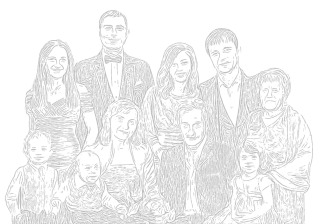
\includegraphics[width=\textwidth]{_cover/to.jpg}
    \emph{Dedicated to my Family}\\
  \end{minipage}
\end{figure}
~
\vspace{2cm}

\noindent The purpose of this book is not merely to instruct but to embark on a shared journey into the realm of 
platform-agnostic application development using Flutter. I've started that book by knowing nothing about Flutter and 
Dart, and the spent time have given me just an initial impulse to the mastery, but I still have something to share with 
you. 

\vspace{3mm}

\noindent I am confident that the time spent on coding (approximately 200 hours) can suffice for grasping the 
fundamental concepts of any programming language or framework, regardless of your prior background, as long as you 
progressively tackle more complex tasks while gradually reducing the need for assistance.

\vspace{3mm}

\noindent My approach to learning has evolved into a day-to-day habit, which I've diligently followed over the past 
20 years while working as a full-stack developer. My technical proficiency is complemented by a profound customer 
focus and business acumen. That possess insights into a product, project, and software life cycles.

\vspace{3mm}

\noindent I warmly invite you to join this project as it unfolds throughout the pages of this book. Together, we will 
embark on an exploration of Flutter and its extensive capabilities. This collaborative learning journey promises to 
be both exciting and enriching as we delve further into the depths of this versatile framework.

%\texttt{Contributors:}
%Viachaslau Lyskouski, ...

\vspace{1cm}

%% Required by lulu.com distribution
%\begin{minipage}{0.15\textwidth}
%  
\includegraphics[width=\textwidth,left]{_cover/lulu-ISBN}
%\end{minipage}
%\hfill
%\begin{minipage}{0.84\textwidth}
%  \emph{\tiny \copyright Viachaslau Lyskouski, 2023: Creative Commons Attribution-\\
%  NonCommercial-NoDerivatives 4.0 International (CC BY-NC-ND 4.0)}
%\end{minipage}

\noindent \emph{\small \copyright Viachaslau Lyskouski, 2023: Creative Commons Attribution-NonCommercial-NoDerivatives 
4.0 International (CC BY-NC-ND 4.0)}

\newpage
\thispagestyle{empty}
~